\section{Diskussion}
\label{sec:Diskussion}
Für die Verdampfungswärme wurde ein Wert von $L = 32,92 \pm 0,43 \cdot 10^3 \, \mathrm{\frac{J}{mol}}$ ermittelt.
Der Literaturwert liegt bei $L_{Literatur} = 40,7 \cdot 10^3 \, \mathrm{\frac{J}{mol}}$ (s. \cite{verdampf}).
Der Literaturwert ist also um 23,63 \% größer als der experimentell bestimmte Wert.\\
Da die Messreihe bis 1 bar aufgrund von Fehlern an unserer Apparatur, von einer anderen Gruppe übernommen wurde, lässt sich relativ wenig
über mögliche Fehlerquellen sagen. Dennoch könnte die Annahme, dass L in dem zu messenden Bereich fast konstant ist, die entstandene Abweichung
erklären.\\
Für die Messung von 1 bar bis 15 bar lässt sich anmerken, dass das Manometer bei steigendem Druck immer wieder nach unten ausgeschlagen hat, um 
dann periodisch um einen Wert zu oszillieren. Dies spricht für eine Undichtigkeit in der Apparatur.\\
Da L im Punkt K.P. konstant sein muss, kommt nur Abbildung \ref{fig:plot3} als physikalisch sinnvoll in Frage.
\newpage

\section{Messdaten}
\label{sec:Messdaten}

\begin{figure}
  \centering
  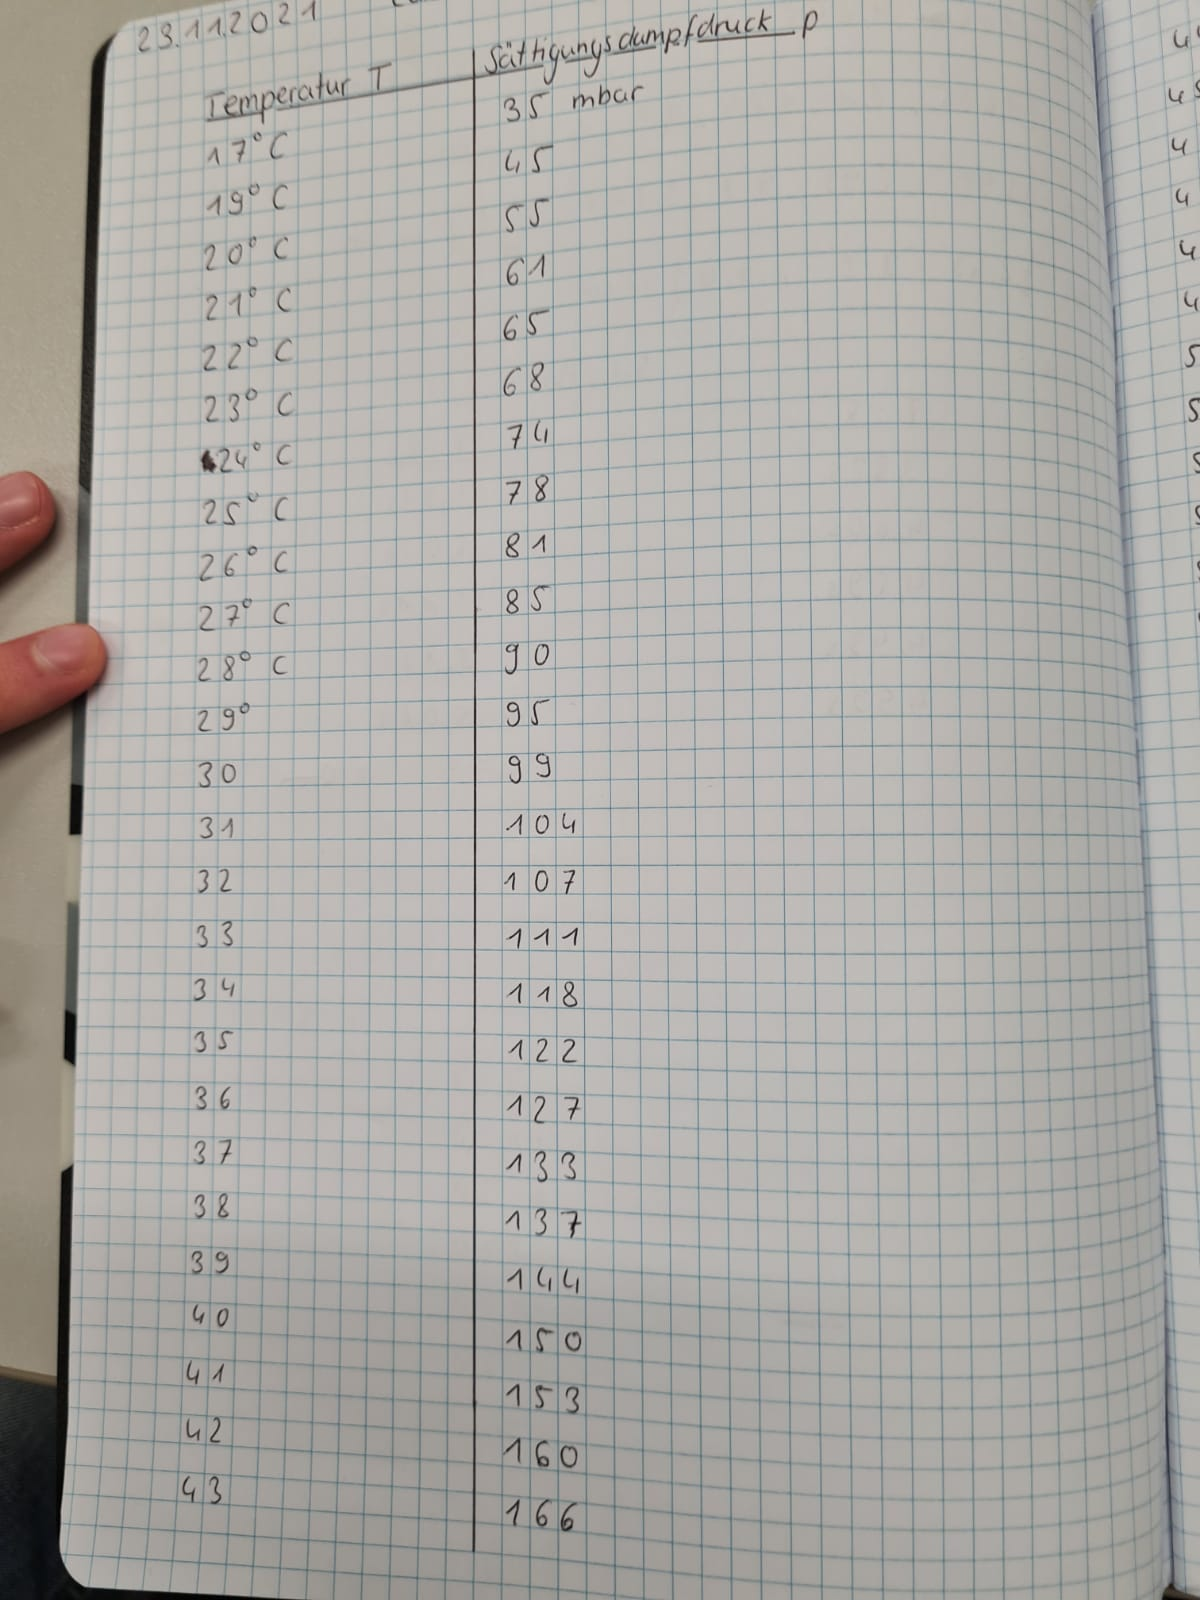
\includegraphics[width=0.7\textwidth]{Messdaten1.jpg}
  \caption{Messdaten Teil 1}
  \label{fig:M1}
\end{figure}

\begin{figure}
    \centering
    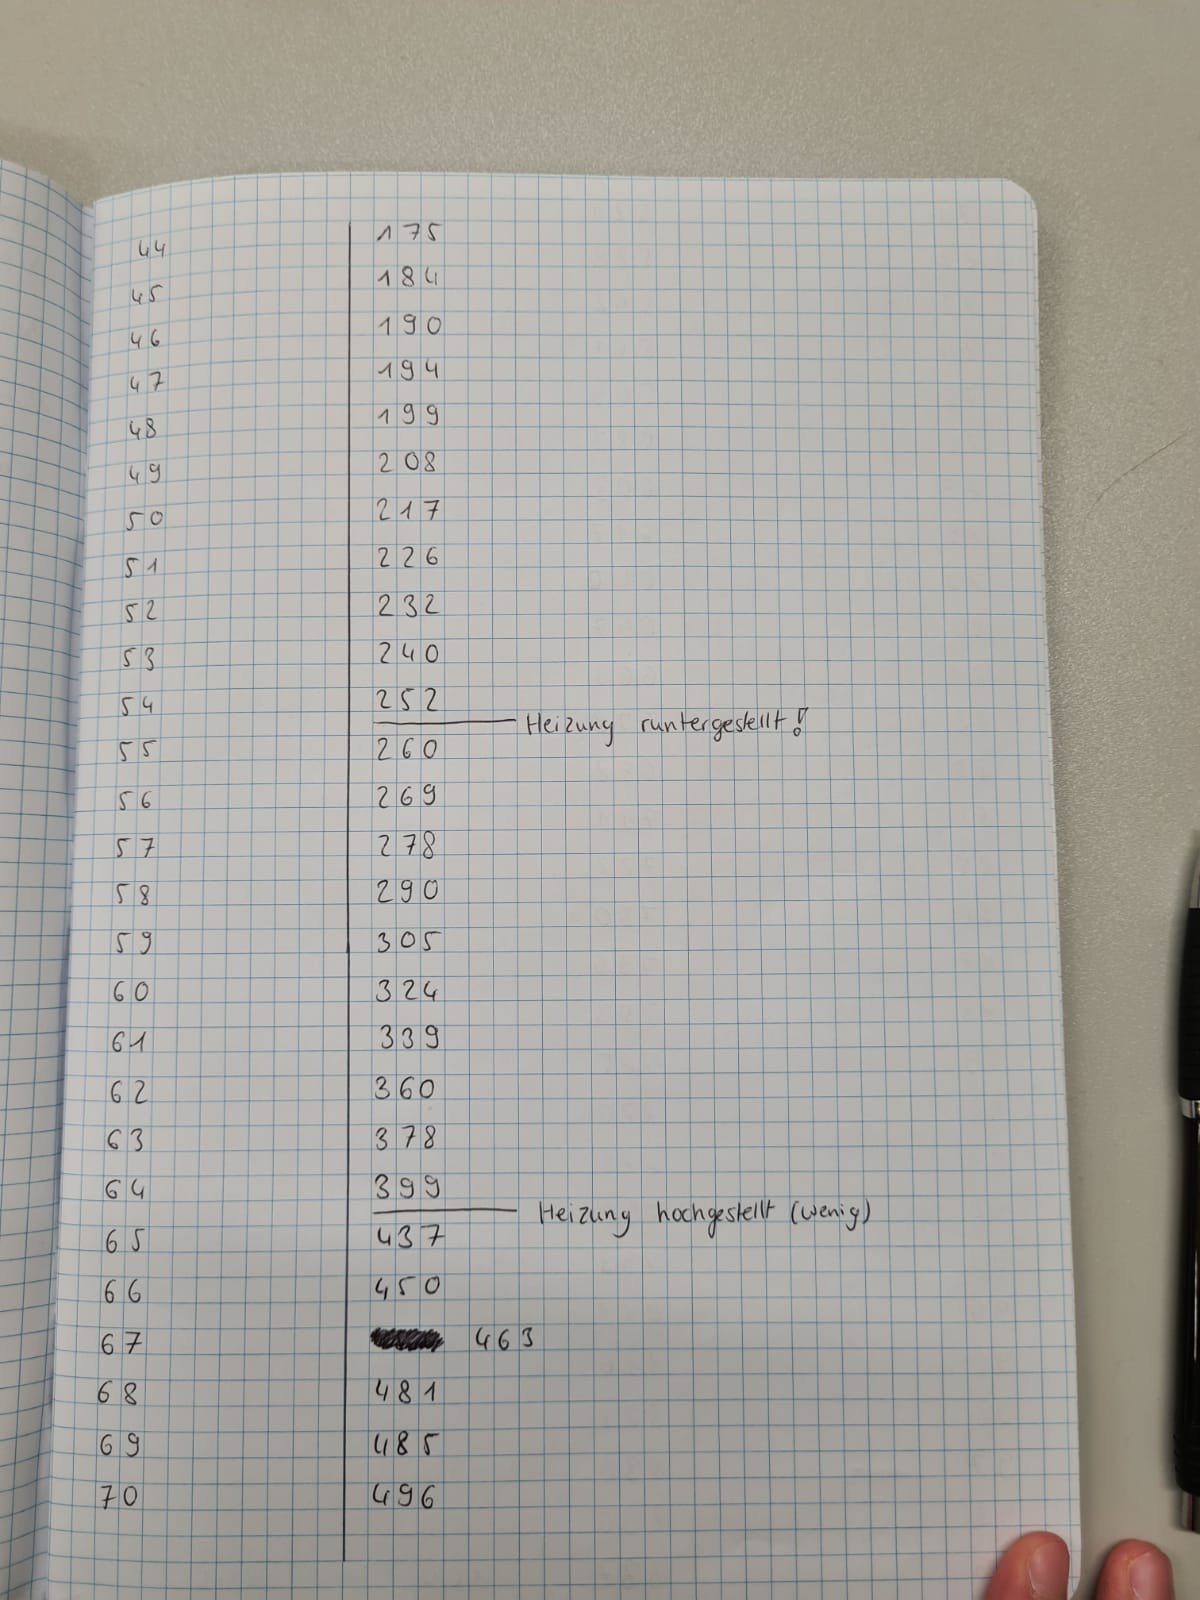
\includegraphics[width=0.7\textwidth]{Messdaten2.jpg}
    \caption{Messdaten Teil 2}
    \label{fig:M1}
\end{figure}

\begin{figure}
  \centering
  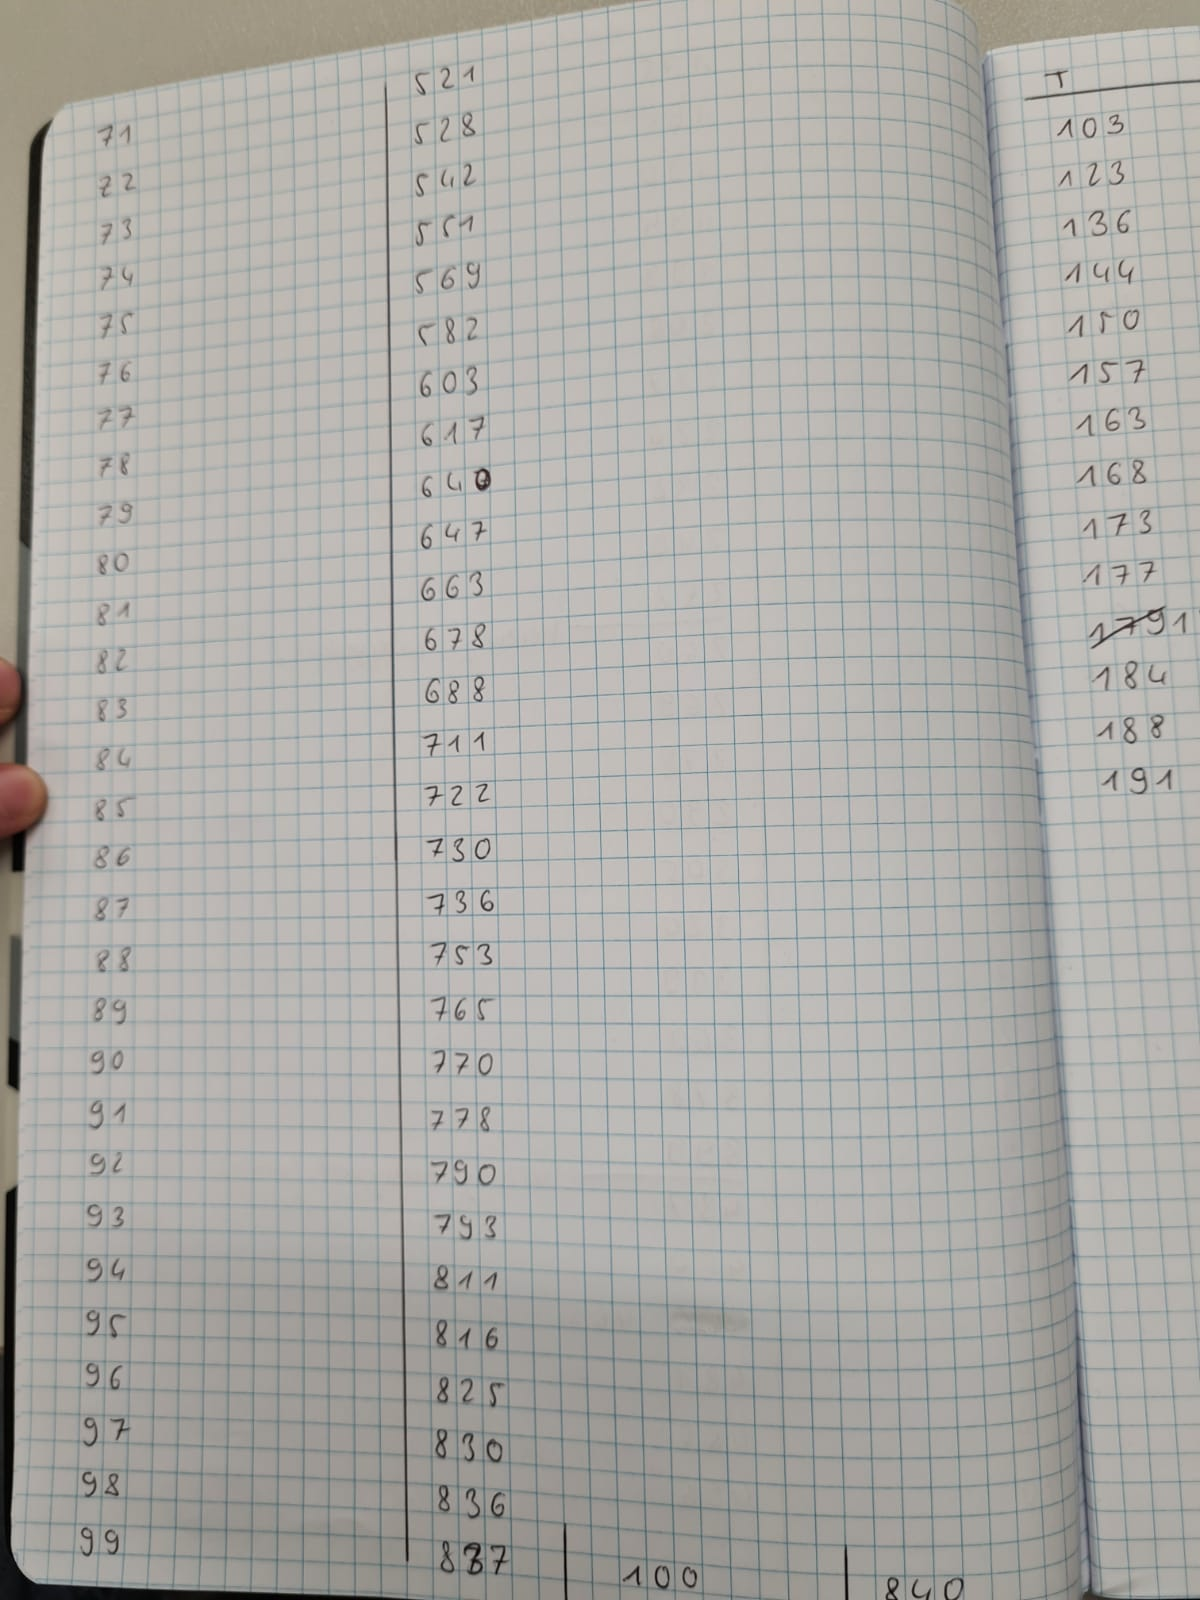
\includegraphics[width=0.7\textwidth]{Messdaten3.jpg}
  \caption{Messdaten Teil 3}
  \label{fig:M1}
\end{figure}